\section{Empirical Results on Dictionary Optimization \label{appendix:gd_interference}}

In \Cref{sec:one-step-proofs}, we considered the performance of threshold and top-$k$ decodings at recovering a subset from a superposition code with a \textit{random} dictionary $F$. One natural question is whether these one-step decodings can do better if the dictionary is optimized to reduce the scale of ``crosstalk'' between distinct codewords.

Of course, when $d \ge N,$ we can make the codewords $f_i$ exactly orthogonal. For this reason, the performance of one-step decodings shown in the left-most column of \Cref{fig:one-step} is much worse than is possible; we never need more than $N$ dimensions to store a latent vector of dimension $N.$ However, when the ratio $d/N$ is small---say, smaller than $1/10$---we conjecture that optimizing the dictionary gives practically no improvement over a random initialization. Unfortunately, we are not aware of a theoretical justification for this fact.

To understand our conjecture, recall the ``crosstalk'' terms
$$
	\xi_i = \sum_{j \neq i} Y_j \langle f_i, f_j \rangle.
$$
For each $i \in [N],$ this is a sum of between $k$ and $(k - 1)$ numbers drawn without replacement from the sequence
$$
	(\langle f_i, f_j \rangle)_{j \neq i}.
$$
Let's fix the dictionary $F$ and consider the empirical distribution defined by this sequence of $N - 1$ numbers. Suppose this distribution has zero mean and variance
$$
	\gamma_i(F) = \frac 1 {N - 1} \sum_{j \neq i} \langle f_i, f_j \rangle^2.
$$
When $k$ is moderately large but much smaller than $N,$ we expect the crosstalk $\xi_i$ to behave like a centered Gaussian with variance $k \gamma_i.$ Specifically, we expect that the probability of its tail events with respect to the random set $Y$ will be governed by the product $k \gamma_i.$ If we assume that tail events for the different variables $\xi_i$ are ``sufficiently independent,'' we conclude overall that the typical value of $\gamma_i(F)$ is the limiting factor for the reliability of one-step estimates.

A dictionary chosen to make the quantities $\gamma_i$ uniformly smaller would, in particular, have smaller average squared interference
$$
	\gamma(F) = \frac 1 N \sum_{i = 1}^N \gamma_i = \binom{n}{2}^{-1} \sum_{i \neq j} \langle f_i, f_j \rangle^2
$$
between distinct codewords. For a random dictionary $F,$ $\gamma(F)$ equals $1/d$ in expectation. Can we decrease this value significantly by optimization?


\begin{figure}[h]
	\begin{center}
		\centerline{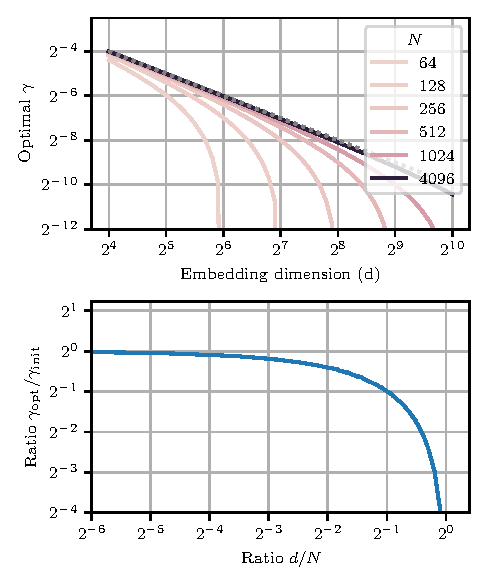
\includegraphics[width=230pt]{figures/gd_interference}}
		\caption{\textbf{Top}: The mean squared interference $\gamma(F)$ of a dictionary $F$ obtained by running projected gradient descent to convergence. The dotted line shows $\gamma_{\text{init}} = 1/d,$ the mean squared interference attained in expectation by a random initialization. The best interference for $N = 2^{16}$ found by gradient descent (not graphed) is nearly indistinguishable from the dotted line. \textbf{Bottom}: A plot of ratio $\gamma_{\text{opt}}/ \gamma_{\text{init}}$ by which gradient descent improves $\gamma$ relative to its expected value at initialization against the ratio $d/N$ between codeword dimension and dictionary size.}
		\label{fig:gd-interference}
	\end{center}
\end{figure}

Using projected gradient descent, we minimized $\gamma(F)$ subject to the constraint of maintaining unit norm codewords. We tested dictionaries with between $N = 64$ and $N = 2^{16} = 65536$ codewords and with codeword dimensions between $d = 16$ and $1024$. In each case, we initialized with a random Rademacher dictionary and optimized to convergence with standard criteria. Our results are shown in \Cref{fig:gd-interference} of \Cref{appendix:gd_interference}.

As $d$ approaches $N,$ we find that the optimal value $\gamma_\text{opt}$ of $\gamma(F)$ converges to $0,$ as expected. On the other hand, when $d \ll N,$ $\gamma_\text{opt}$ is very close to $1/d,$ its expected value under a random initialization. For example, with $N = 2^{16}$ (not plotted), the optimal value of $\gamma(F)$ is indistinguishable from $1/d$ on a log-log plot.

Furthermore, we find a striking regularity. Empirically, the ratio $\gamma_\text{opt} / d^{-1} = d \gamma_\text{opt}$ between the optimal value of $\gamma$ and its expected value at initialization turns out to be a function of the relative dimension $d/N.$ Since this holds as $N$ ranges over several orders of magnitude, it is natural to believe it may hold in general.

\begin{claim}
	For given $(N, d),$ the optimal value of $\gamma(F)$ for a dictionary $F \in \R^{d \times N}$ of unit norm codewords iso
	$$
		\gamma_\text{opt}(N, d) = \frac{\kappa(d/N)}{d}
	$$
	for some function $\kappa.$ Furthermore, $\kappa(r)$ is close to $1$ for small values of $r.$
\end{claim}

If true, this means that the values $\gamma_i(F)$ governing the scale of crosstalk suffered by matched filters can't be made significantly smaller than $1/d$ when $d \le \epsilon N$ for small $\epsilon.$

We're not aware of theoretical results in this direction. Note in particular that this is not obviously related to work on sphere packing (see \cite{cohn_sphere_2014}) since we are interested in the \textit{scale} of the distribution of inner products rather than in maximum values.
